\documentclass{package/fancy-book}
\setlength{\parindent}{2em}
\usepackage[UTF8]{ctex}

%%%%%%%%%% Default Package %%%%%%%%%%%%%
\usepackage{package/color-env}
\usepackage{package/quiver}
\usepackage{background}
\usepackage[object=vectorian]{pgfornament} %% used in title.tex
\usepackage{calligra} %%% (optional) to make the Title text beautiful 
\usepackage{lipsum}  %% for dummy text 
\usepackage{amssymb,amsmath,amsfonts}  %%% for maths

%%%%%% Optional Packages %%%%%%%
\usepackage{lettrine} %% for nice looking 
\usepackage{GoudyIn} %% first Letter of the paragraph
\renewcommand{\LettrineFontHook}{\color{black}\GoudyInfamily{}}
\LettrineTextFont{\itshape}
\setcounter{DefaultLines}{3}%
%%%%%%%%%%%%%%%%%%%%%%%%%%%%%%%%%%%%%

\usepackage{fourier-orns}
\newcommand{\ornamento}{\vspace{2em}\noindent \textcolor{darkgray}{\hrulefill~ \raisebox{-2.5pt}[10pt][10pt]{\leafright \decofourleft 
\decothreeleft  \aldineright \decotwo \floweroneleft \decoone   \floweroneright 
\decotwo \aldineleft\decothreeright \decofourright \leafleft} ~  \hrulefill \\ \vspace{2em}}}

%定义命令
\newcommand{\N}{\mathbb{N}}
\newcommand{\Z}{\mathbb{Z}}
\newcommand{\Q}{\mathbb{Q}}
\newcommand{\R}{\mathbb{R}}
\newcommand{\C}{\mathbb{C}}
\newcommand{\HH}{\mathbb{H}}
\newcommand{\RP}{\mathbb{RP}}

%单标号
\newenvironment{singlealign}{\align\renewcommand{\\}{\nonumber\newline}}{\endalign}

%%%% Bibliography %%%%%%%%%
% Required packages are included in notes class
% Can be tweaked in the notes.cls file itself
\addbibresource{resource/references.bib}


\begin{document}
\begin{titlepage}

%%%%%%%%%%%%%%%%%%%%%%%%%%%%%%%%%%%% Inspired From  %%%%%%%%%%%%%%%%%%%%%%%%%%%%%%%%%%%%%%%%%%%%%%%%% 
%%%%  https://www.reddit.com/r/LaTeX/comments/j9d739/hello_world_in_latex_is_a_lot_cooler/   %%%%%
%%%%%%%%%%%%%%%% If this doesn't look nice then you may remove it %%%%%%%%%%%%%%%%%%%%%%%%%%

\backgroundsetup{
scale=1,
opacity=1,
angle=0,
color=black,
contents={
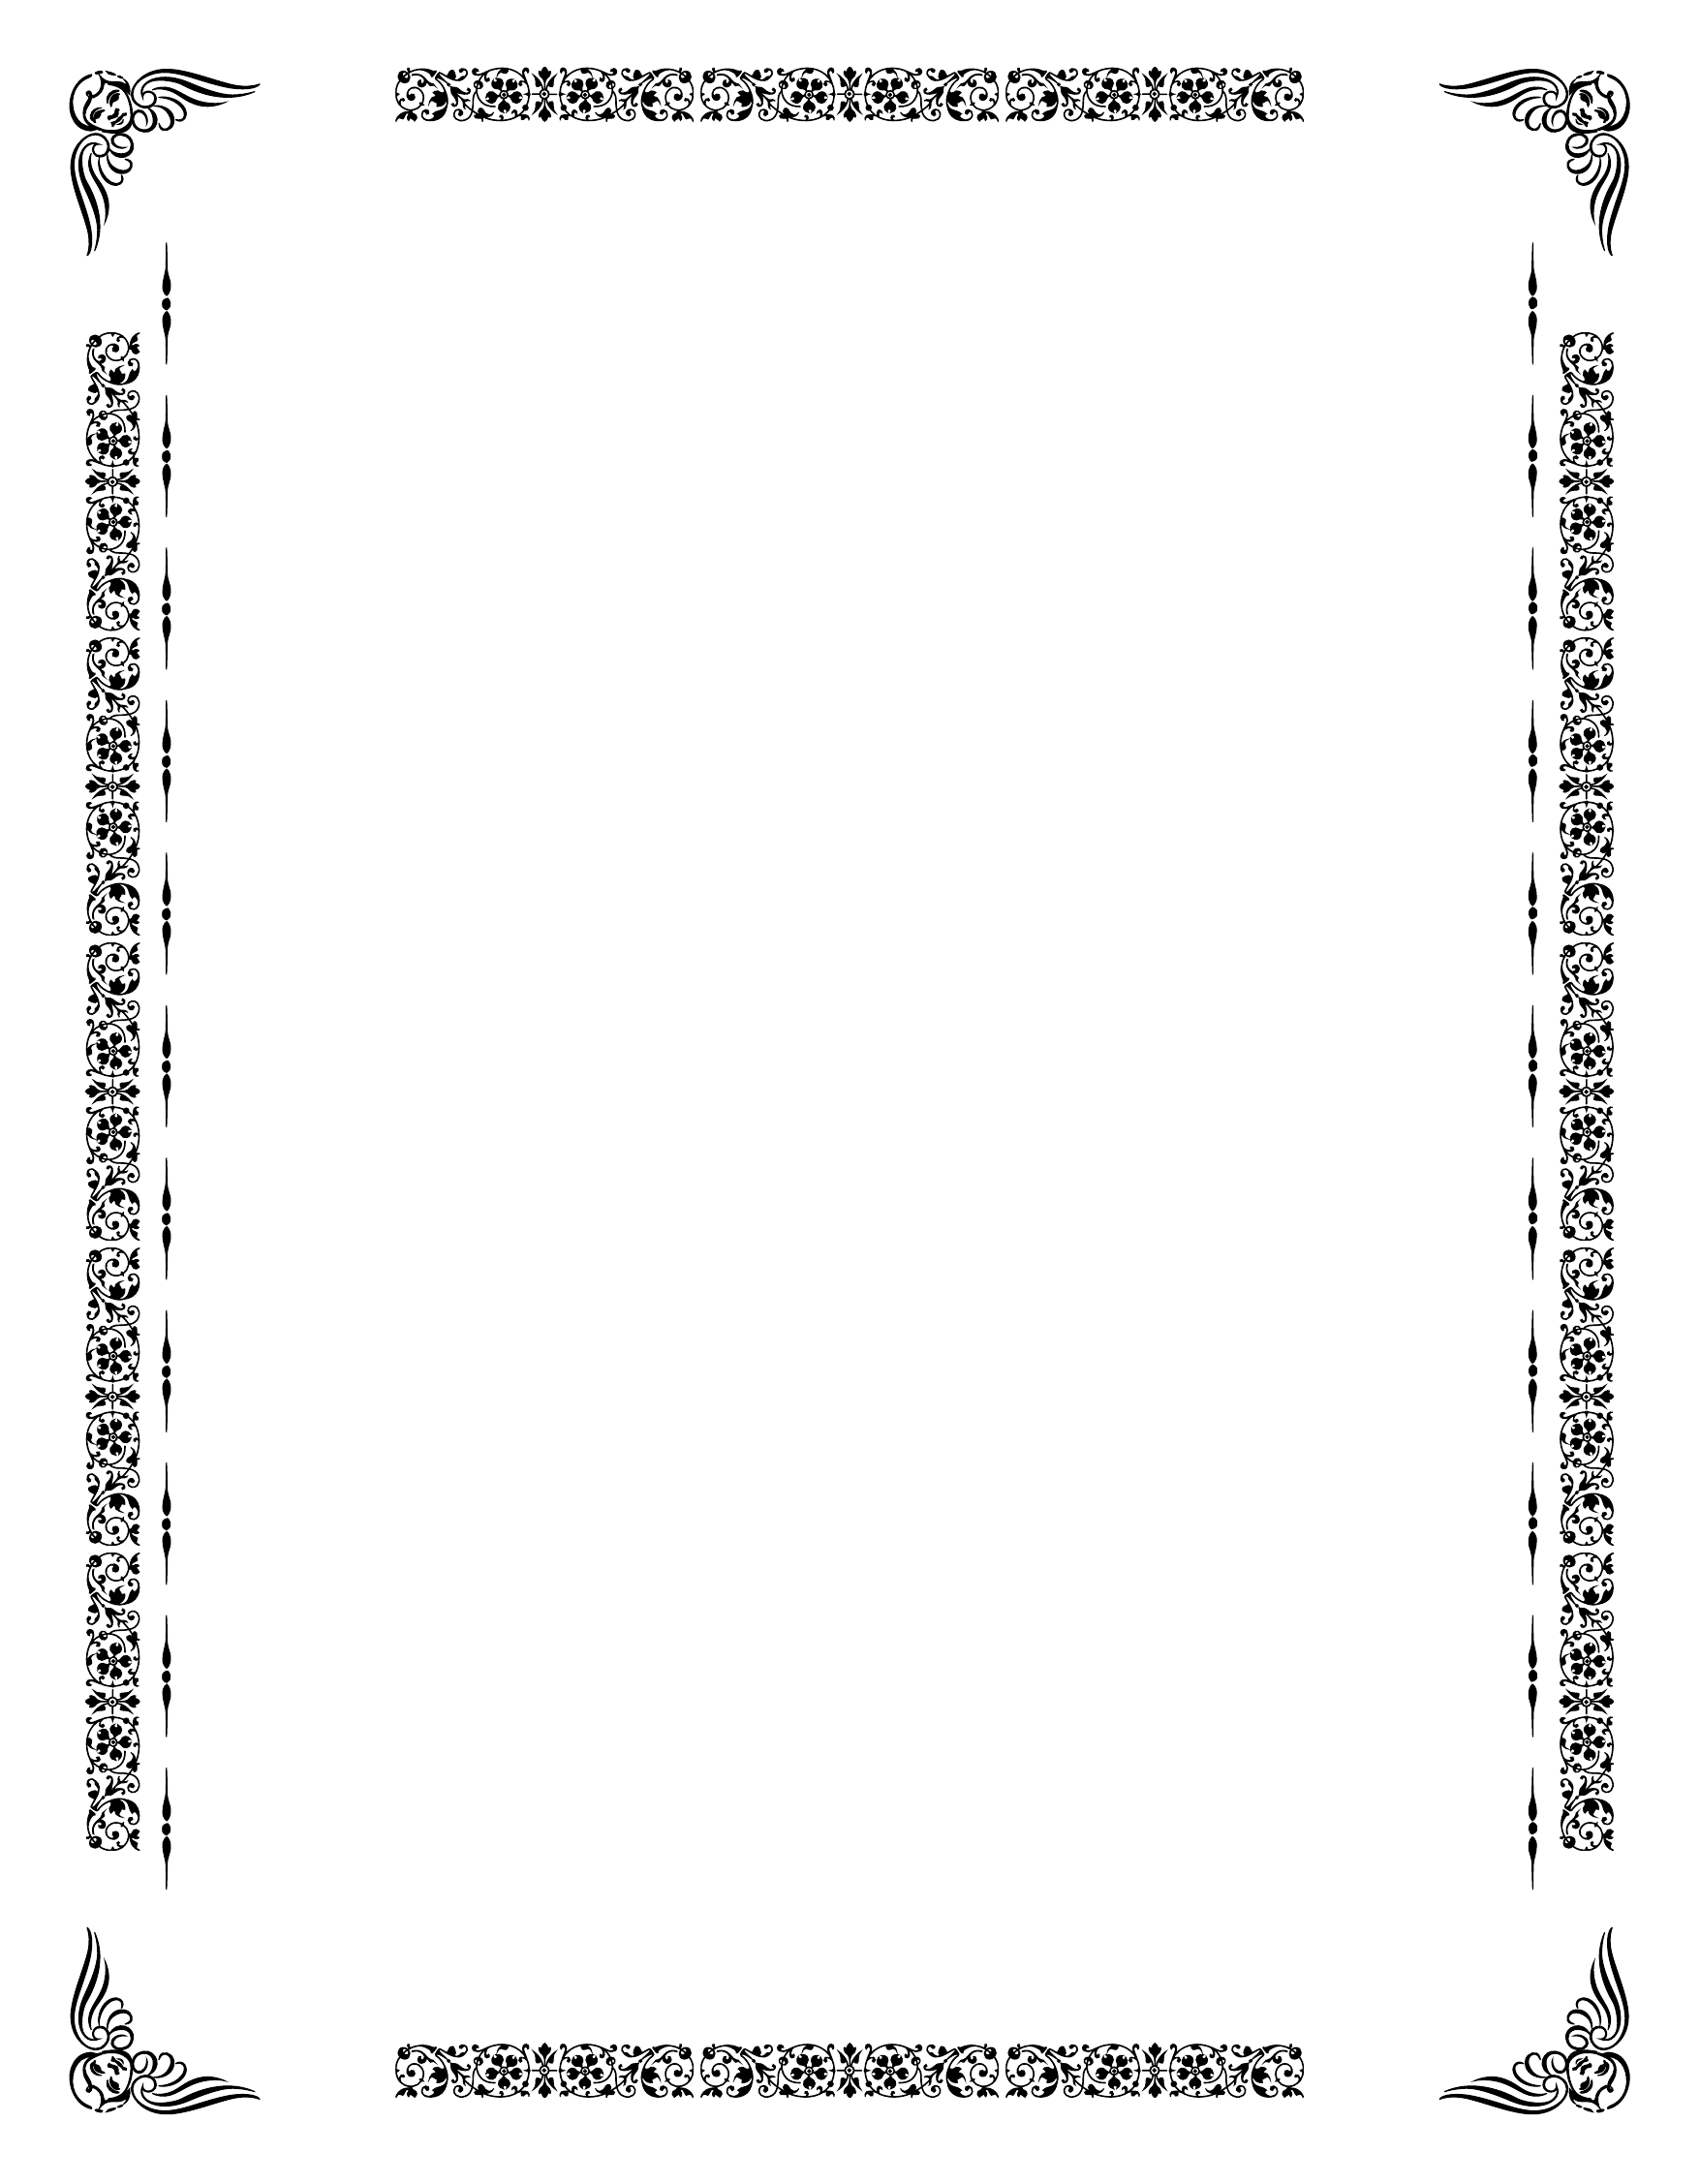
\begin{tikzpicture}[color=black, every node/.style={inner sep= 15pt}]
\node (NW) [anchor=north west] at (current page.north west){\pgfornament[width=2.5cm] {131}};
\node (NE) [anchor=north east] at (current page.north east){\pgfornament[width=2.5cm, symmetry=v]{131}};
\node (SW) [anchor=south west] at (current page.south west){\pgfornament[width=2.5cm, symmetry=h]{131}};
\node (SE) [anchor=south east] at (current page.south east){\pgfornament[width=2.5cm, symmetry=c]{131}};
\foreach \i in {-4,0,4}
\node[anchor=north,xshift=\i cm] at (current page.north){\pgfornament[scale=0.25,symmetry=v]{71}};
\foreach \i in {-4,0,4}
\node[xshift=\i cm, yshift=32.25 pt] at (current page.south){\pgfornament[scale=0.25,symmetry=v]{71}};
\foreach \i in {-8,-4,0,4,8}
\node[yshift=\i cm, xshift=32.25pt, rotate=90] at (current page.west){\pgfornament[scale=0.25,symmetry=v]{71}};
\foreach \i in {-8,-4,0,4,8}
\node[yshift=\i cm, xshift=-32.25pt, rotate=90] at (current page.east){\pgfornament[scale=0.25,symmetry=v]{71}};
\foreach \i in {-11,-9,...,7,9}
\node[anchor=west, yshift=\i cm, xshift=52.25pt, rotate=90] at (current page.west){\pgfornament[scale=0.1]{80}};
\foreach \i in {-11,-9,...,7,9}
\node[anchor=east, yshift=\i cm, xshift=-52.25pt, rotate=-90] at (current page.east){\pgfornament[scale=0.1]{80}};
\end{tikzpicture}
}}

%%%%%%%%%%%%%%%%%%%%%%%%%%%%%%%%%%%%%%%%%%%%%%%%%%%%%%%%%%%%%%%%%%%%%%%%%%%%%%%%%%%%%%%%%%%%%%%%%%%%%%%%%%%%%%%%%%

\centering % Centre everything on the title page
		
\scshape % Use small caps for all text on the title page

\vspace*{\baselineskip} % White space at the top of the page

%------------------------------------------------
%	Title
%------------------------------------------------

\rule{\textwidth}{1.6pt}\vspace*{-\baselineskip}\vspace*{2pt} % Thick horizontal rule
\rule{\textwidth}{0.4pt} % Thin horizontal rule

\vspace{0.75\baselineskip} % Whitespace above the title

{\huge \calligra{\textbf{Note for Homological Algebra} }\\} % Title

\vspace{0.75\baselineskip} % Whitespace below the title

\rule{\textwidth}{0.4pt}\vspace*{-\baselineskip}\vspace{3.2pt} % Thin horizontal rule
\rule{\textwidth}{1.6pt} % Thick horizontal rule

\vspace{2\baselineskip} % Whitespace after the title block

%------------------------------------------------
%	Subtitle
%------------------------------------------------

\Huge{范畴论笔记} 

\vspace*{3\baselineskip} % Whitespace under the subtitle



\vspace{0.5\baselineskip} 

{\scshape   \LARGE Edited by\\  颜成子游/南郭子綦} % Editor list
\vspace{0.2\baselineskip} 


\vfill 
\Large{最后一次编译时间:\DTMnow}
%------------------------------------------------
% Author
%------------------------------------------------

\begin{figure}[!h]
    \centering
    
\includegraphics[width = 3cm, height= 3cm]{resource/icon.png}%% include the university icon here
\end{figure}
\vspace{0.3\baselineskip} 

\end{titlepage}
\backgroundsetup{contents={}} %% to remove background and watermark from other pages
\tableofcontents

\quad

学习数学的时候,无论是逛贴吧,看论坛,还是水群,亦或是读一些有意思的小推送,以及看一些没有时间记录的note的时候,总能遇到一些非常值得记录的小知识。这些知识或是结论,或是定义和思想,或是目前前沿的进展。

本篇pdf的目的就是为了记录这些知识。每一条知识我们都会用时间标注。笔者一是为了记录自己的数学学习之路,二也是为了让自己零碎化的数学学习有更好的效果。

笔者目前从事微分几何方向的研究生学习
\chapter{几何}
\section{微分流形}
这里整理的是微分流形中老是记不住的东西。
\begin{proposition}[流形的微分结构]{manifold-structure}
    一个流形上可能赋予不同的微分结构,并且这样的微分结构可能是不微分同胚的!比如,Milner证明了$S^7$上存在着不微分同胚的微分结构。当然,也存在完全没有微分结构的流形。
\end{proposition}
\subsection{子流形}
下面这个定理是司空见惯的。但是无奈我每次都记不住证明(缺乏一个好的感知)
\begin{theorem}[正则子流形的标准形式]{submanifold}
    设$M^m$是$N^n$的正则子流形。这等价于说$M$是$N$的子拓扑空间,并且对于任意$p \in M$,存在$p$在$N$中局部坐标邻域$U$和坐标函数$\{x^1,\dots,x^n\}$使得:
    \begin{equation}
        M \cap U=\{q \in U|x^i(q)=0,m+1\leq i \leq n\}
    \end{equation}
\end{theorem}
\begin{proof}
    我们需要用到浸入子流形的标准形式(证明用到逆映射定理)这里不再赘述。

    假设$M$是$N$的正则子流形,则$i:M \to N$是嵌入映射。任取$p \in M$,在$M$上和$N$上分别有$U,\phi$和$V,\psi$作为坐标邻域使得$U \subset V$.

    考虑映射$\psi \circ \phi^{-1}:\R^m \to \R^n$.根据浸入的标准形式,有$(x^1,\dots,x^m) \mapsto (x^1,\dots,x^m,0,\dots,0)$。

    因为$M$是$N$的子拓扑空间,所以可以取$N$中含$p$的开邻域$U_1 \subset V$使得$M \cap U_1 = U$.

    我们把$V$上的坐标限制在$U_1$上,作为其坐标映射。当$q \in M \cap U_1$时,$q \in U$.所以$x^i(q)=0,m+1\leq i \leq n$.于是$M \cap U_1\subset \{x^i(q)=0,m+1\leq i \leq n\}$.

    另一方面,设$q \in U_1$且$x^i(q)=0,m+1\leq i \leq n$.

    记$q'=\varphi^{-1}(x^1(q),\dots,x^m(q))$,则:
    \begin{align}
        \psi(q')&=\psi \circ \varphi^{-1}(x^{1}(q),\dots,x^m(q))\\&=(x^1(q),\dots,x^m(q),0,\dots,0)\\&=(x^1(q),\dots,x^m(q),x^{m+1}(q),\dots,x^n(q))\\&=\psi(q)
    \end{align}
    这说明$q=q' \in U \subset M$.

    如果$M$满足定理陈述,首先在$M$上取子拓扑。其次只需要把$M$的局部坐标定义为$M \cap U$上的前$m$个分量即可。
\end{proof}
\begin{theorem}[常秩定理]{constant-rank}
    设$f:M \to N$为光滑映射。存在$l>0$使得$\mathrm{rank}_p f=l$,$\forall p \in M$,则对于每个固定的$q \in N$,$q$在$f$的原像$f^{-1}(q)$要么为空集,要么为$M$的正则子流形,其维数为$m-l$。
\end{theorem}
\begin{proof}
    设$S=f^{-1}(q)$。根据定理\ref{submanifold},我们将证明存在$p$附近$M$上局部坐标$U,\varphi$和$q$附近$V,\psi$使得$\phi(p)=0 \in \R^m$,$\psi(q)=0 \in \R^n$,$f(U) \subset V$,且$f$的局部表示为$\psi \circ f \circ \varphi$形如:
    \begin{equation}
        \psi \circ f \circ \varphi(x^1,\dots,x^m)=(x^1,\dots,x^l,g^{l+1}(x^1,\dots,x^l),\dots,g^n(x^1,\dots,x^l))
    \end{equation}

    由于是完全局部的问题,所以设$M$为$\R^m$,$N$是$\R^n$。$f$可表示为:
    \begin{equation}
        f(x^1,\dots,x^m)=(f^1,\dots,f^n)
    \end{equation}
    矩阵:
    \begin{align}
        (\frac{\partial f_i}{\partial x^j})
    \end{align}
     秩为$l$。不妨设前$l$行,$l$列非退化。定义$g:\R^m \to \R^m$为:
     \begin{align}
        g(x^1,\dots,x^m)=(f_1,\dots,f_l,x^{l+1},\dots,x^{m})
     \end{align}
     从而$g$的Jacobi矩阵非退化。根据逆映射定理,存在$0$处的开邻域$U$和$V$使得$g|_U :U \to V$是微分同胚。于是$\varphi:=g|_U$是$0$处的坐标映射。$f$在该坐标的表示为$f \circ \varphi^{-1}$:
     \begin{align}
        f \circ \varphi^{-1}(x^1,\dots,x^m)=(x^1,\dots,x^l,g^{l+1},\dots,g^n)
     \end{align}
     $\mathrm{rank}J(f \circ \varphi^{-1})|_V=l$。所以$g^i$对$x^j$的偏导为$0$,$l+1\leq i \leq n,l+1 \leq j \leq m$。

     所以$g^i=g^i(x^1,\dots,x^l)$证毕。

     于是
     \begin{align}
        S \cap U=\{s \in U|f(s)=0\}=\{s \in U|x^1(s)=\dots=x^l(s)=0,g^j(x^i(s))=0\}=\{s \in U|x^1(s)=\dots=x^l(s)=0\}
     \end{align}

\end{proof}
这里注意的是,如果$f^{-1}(q)$的某个开邻域内$\mathrm{rank}f$是常数,则可以说明$f^{-1}(q)$是正则子流形。但是矩阵微扰的情况下不会变小。因此只要$\mathrm{rank}f$在$f^{-1}(q)$上恒为$n$(最大可能的秩)即可找到这个开邻域,从而$f^{-1}(q)$是$m-n$维的正则子流形。此时也称$q$是$f$的正则值。
\subsection{横截相交}
横截相交这里,是老是记不住:1.稳定性 2.正则子流形的生成。
\begin{definition}[横截相交]{directly}
    设$f:M \to N$是光滑的。若$S$是$N$的\textbf{正则子流形},且对于任意满足$f(p)=q \in S$的$p\in M$,都有:
    \begin{equation}
        f_*(p)(T_pM)+T_q(S)=T_q(N)
    \end{equation}
    则称$f$和$S$横截相交,记作$f \pitchfork S$。若$f(M)\cap S=\emptyset$也称横截相交。
\end{definition}
显然正则值$q$处$M$与$N$横截相交。
\begin{lemma}{}
    设$0$是$g:N \to \R^k$的正则值,且$S=g^{-1}(0)$.则$f:M \to N$和$S$横截相交当且仅当$0$是$g \circ f$的正则值。
\end{lemma}
\begin{proof}
    若$0$是正则值,则对于任何$p \in f^{-1}(S)$有$(g \circ f)_{*p}(T_pM)=g_{*f(p)}f_{*p}(T_p M)=T_0 \R^k$。

    注意到$T_{f(p)}S=\ker g_{*f(p)}$,$g_{*f(p)}T_{f(p)}N=T_0\R^k$。则上面的式子与:
    \begin{align}
        T_{f(p)}S+f_{*p}(T_p M)=T_{f(p)}N
    \end{align}
    等价。
\end{proof}
\begin{theorem}{direct-submanifold}
    设$f:M \to N$光滑且$S$是$N$的正则子流形。如果$f \pitchfork S$,则$f^{-1}(S)$是$M$的正则子流形且:
    \begin{align}
        \mathrm{dim}M-\mathrm{dim}f^{-1}(S)=\mathrm{dim}N-\mathrm{dim}D
    \end{align}
\end{theorem}
\begin{proof}
    设$p \in f^{-1}(S)$。记$q=f(p)$。因为$S$是正则子流形,根据$S$的结构定理,存在$q$在$N$中的局部坐标邻域$U_q$以及淹没$g:U_q \in \R^k$($k=\mathrm{dim}N-\mathrm{dim}S)$。使得:
    \begin{align}
        S \cap U_q=g^{-1}(0)
    \end{align}
    注意到$0 \in \R^k$是$g \circ f$的正则值,则存在$p$的开邻域$f^{-1}(U_q)$中的$f^{-1}(S)$为正则子流形,维数为$\mathrm{dim}M-k=\mathrm{dim}M-\mathrm{dim}N+\mathrm{dim}S$。
\end{proof}
显然,用$\mathrm{codim}f^{-1}(S)=\mathrm{codim}S$来表述上面的定理更方便。

\begin{theorem}[横截相交的稳定性]{transversal-stability}
    设$M,P,S,N$是微分流形。其中$M$紧致,$S$是$N$的闭正则子流形。设$f$是$M \times P \to N$的光滑映射,取$p \in P$,定义$f_p:M \to N$,$f_p(x)=f(x,p)$,则集合:
    \begin{align}
        \Omega=\{p \in P|f_p\text{ is transversal to  }S\}
    \end{align}是开集。
\end{theorem}
\begin{proof}
    设$p_0 \in \Omega$.我们需要说明对于$p_0$附近的点$p$,$f_p$与$S$也横截相交。若不然,存在$p_i \in P$使得$p_i \to p_0$且$f_{p_i}$与$S$不横截相交。因此存在$x_i \in M$使得$f(x_i,p_i)=y_i \in S$且:
    \begin{align}
        f_{*(x_i,p_i)}(T_{x_i}M)+T_{y_i}S \neq T_{y_i}N
    \end{align}
    $M$紧致,所以$x_i$收敛于$x_0$。从而$(x_i,p_i)\to (x_0,p_0)$。$S$是闭集,则$f(x_0,p_0)\in S$。$S$是正则子流形,于是存在$y_0$的局部坐标邻域$V$和光滑淹没$\psi:V \to \R^k$。因为$f_{p_0}$与$S$横截相交,则$0$是$\psi \circ f(\cdot,p_0)$的正则值。

    从而$i$足够大的时候,可以得到$\psi \circ f(\cdot,p_i)$也拥有$0$为正则值,且$y_i \in V$。这矛盾于$p_i \notin \Omega$。
    
\end{proof}
\subsection{Sard定理}
\begin{lemma}[Zero-measure]{}
    $\R^n$上的Lipschitz映射把零测集映射为零测集。$C^1$也是。
\end{lemma}
\begin{definition}{singular-p}
    对于$f:M \to N$,如果$p \in M$处$f_{*p}$不是满射,则称$p$是$f$的临界点.临界点的像称为临界值。
\end{definition}
\begin{theorem}[Sard定理]{Sard}
    设$f:M \to N$是微分流形之间的光滑映射。则$f$的临界值是$N$的零测集。
\end{theorem}
\begin{proof}
    证明的思路是用$k$阶偏导数全为$0$的集合来逐步逼近$C$($C$是临界值集合)。每次都只会增加一个零测的集合,而导数阶数足够大的时候,本来只有零测集合。从而得到证明。
\end{proof}
我们用Sard讨论一些应用。
\begin{lemma}{}
    $f:M \times P \to \R^k$是光滑的.$0$是$f$正则值,则集合:
    \begin{align}
        \{p \in P|0\text{ is a singular image of }f_p\}
    \end{align}
    是$P$的零测集。
\end{lemma}
\begin{proof}
    定义$\pi:M \times P \to P$。设$S=f^{-1}(0)$。把$\pi$限制在$S$上。
    
    则$0$是$f_p$的正则值当且仅当$p$是$\pi|_S$的正则值。
\end{proof}
\begin{theorem}[横截性定理]{transversal}
    $f:M \times P \to N$是光滑的.$Z$是$f$正则子流形,则集合:
    \begin{align}
        \{p \in P|f_p \text{ is not transversal to 
         }Z\}
    \end{align}
    是$P$的零测集。
\end{theorem}
\begin{proof}
    用引理。$Z$可以被$N$至多可数个坐标邻域覆盖。又因为可数个零测集的并还是零测集,所以我们不妨考虑$Z=g^{-1}(0)$,$g:N \to \R^k$是光滑淹没。

    因此$0 \in \R^k$是$g \circ f$的正则值。而$f_p$与$Z$横截相交等价于$0 \in \R^k$是$g \circ f_p$的正则值。因此转化为上一个引理。
\end{proof}
\begin{example}[映射的微扰]{}
    设$f:M \to \R^n$是光滑的,$Z$是$R$的正则子流形。令$F: M \times \R^n \to \R^n$,$f(p,a)=f(p)+a$。

    $F$是淹没!所以与$Z$横截相交。则对于几乎所有的$a \in \R^n$,$f(p)+a:M \to \R^n$都与$Z$横截相交。即对$f$做微小扰动可得横截相交。
\end{example}
\subsection{Frobenius定理}
这个知识点出现在这里的原因是笔者对于这个知识点的熟练度很低。经常出现知道但是忘了的情况。另外,也顺便学一下该定理的外微分形式。
\subsubsection{一般描述}
Frobenius定理的动机是比较干净的。其中一个是向量场的奇点问题。奇点问题本身和流形的拓扑性质密切相关:在偶数维球面上不存在无奇点的光滑切向量场,而环面却存在。

先考虑非奇点处的性状。
\begin{theorem}{nonsingular-vector-field}
    设$X$是$M$上光滑的切向量场。若$p\in M$且$X_p\neq 0$,则存在$p$的一个局部坐标邻域$(W;w^i)$使得:
    \begin{align}
        X|_W=\frac{\partial}{\partial w^1}
    \end{align}
\end{theorem}
\begin{proof}
    先取出$p$的一个局部坐标$(U;u^i)$使得$u^i(p)=0$。$X$限制在$U$可以写为:
    \begin{align}
        X|_U=\sum_{i=1}^m \xi^i \frac{\partial}{\partial u^i}
    \end{align}
    不妨设$\xi^1(p)\neq 0$且$\xi^1$在$U$上处处不为$0$。考虑常微分方程:
    \begin{align}
        \frac{du^\alpha}{du^1}=\frac{\xi^{\alpha}(u^1,\dots,u^m)}{\xi^1(u^1,\dots,u^m)},\alpha=2,\dots,m
    \end{align}
    这里$u^2,\dots,u^m$是欲求的$m-1$个关于$u^1$的函数。根据光滑性,存在正数$\delta$使得$\{(u^1,\dots,u^m)||u^i|<\delta\|\}\subset U$使得任意给定初值$(v^2,\dots,v^m)$,$|v^\alpha|<\delta$,方程就有唯一的解:
    \begin{align}
        u^\alpha=u^\alpha(u^1;v^2,\dots,v^m),-\delta<u^1<\delta
    \end{align}
    并且满足条件:
    \begin{align}
        u^\alpha(0;v^2,\dots,v^m)=v^\alpha
    \end{align}
    于是我们等于是解出了一个变量替换:
    \begin{align}
        u^1=v^1;u^\alpha=u^\alpha(v^1,v^2,\dots,v^m)
    \end{align}
    且Jacobi行列式为$1$。(只要$v^1=0$)。

    所以存在$p$的一个邻域$W \subset U$使得以$v^i$为局部坐标系。在这个坐标系下,我们可以计算:
    \begin{singlealign}
        X|_W&=\sum_{i=1}^m \xi^i \frac{\partial}{\partial u^i} \nonumber\\
        &=\xi^1 \frac{\partial}{\partial u^1}+\sum_{i=2}^m \xi^i \frac{\partial}{\partial u^i} \nonumber\\
        &=\xi^1 \cdot \sum_{i=1}^m \frac{\partial u^i}{\partial v^1}\frac{\partial}{\partial u^1}=\xi^1 \frac{\partial}{\partial v^1}
    \end{singlealign}
    接下来只需要对$\dfrac{dv^1}{\xi^1}$积分即可标准的化出$X$的形式。
\end{proof}
这个问题很容易被推广到多个向量场的情况。这里我们给出一个条件:
\begin{align}
    [X_\alpha,X_\beta]=0
\end{align}

上述条件是比较强的。通常考虑的是下面的类似问题。
\begin{definition}[Distribution]{Distribution}
    设对于每一个$p \in M$我们都制定了一个切空间$T_p$的$h$维子空间$L^h(p)$。若对于每个点$p \in M$,在$p$的一个邻域$U$上存在$h$个处处线性无关的光滑切向量场$X_1,\dots,X_h$,使得$X_i(p)$张成了$L^h(p)$,则称$L^h$是$M$上光滑的$h$维分布,记为:
\begin{align}
    L^h|_U=\{X_1,\dots,X_h\}
\end{align}
\end{definition}
问题是,何时能给出一个分布$L^h$,使得存在局部坐标系$(W,w^i)$且:
\begin{align}
    L^h|_U=\langle \frac{\partial}{\partial w^i}\rangle,i=1,\dots,h
\end{align}
我们稍微分析一下这个条件。比如此时,有:
\begin{align}
    X_\alpha=\sum_{\beta=1}^h a_\alpha^\beta \frac{\partial}{\partial w^\beta}
\end{align}
所以
\begin{align}
    [X_\alpha,X_\beta]=\sum_{\gamma=1}^h C_{\alpha\beta}^\gamma X_\gamma,C_{\alpha\beta}^\gamma=\sum_{\delta,\eta=1}^h(a_\alpha^\delta \frac{\partial a_\beta^\eta}{\partial w^\delta}-a_\beta^\delta\frac{\partial a_\alpha^\eta}{\partial w^\delta})b_\eta^\gamma
\end{align}
其中$b=(b_\beta^\alpha)$表示$a$的逆矩阵。
\begin{definition}[Frobenius条件]{}
    如果$\{X_1,\dots,X_h\}$张成$L^h$(任意邻域$U$上),且对于李括号而言是封闭的,则称该分布满足Frobenius条件。
\end{definition}
\begin{theorem}[Frobenius定理]{Frobenius}
    若有一个定义在$U$上的分布$L^h$,且对于任何$p\in U$,总是存在局部坐标系$(W,w^i)$使得:
\begin{align}
    L^h|_W=\langle \frac{\partial}{\partial w^i}\rangle,i=1,\dots,h
\end{align}
则等价于该分布满足Frobenius条件。
\end{theorem}
\begin{proof}
    考虑数学归纳法。根据之前的叙述,$h=1$的时候定理\ref{nonsingular-vector-field}给出了证明。

    假设$h-1$的时候定理得证。设$L^h$由$U$上处处线性无关的切向量场$X_1,\dots,X_h$生成,并且:
    \begin{align}
        [X_\alpha,X_\beta]\cong 0(\mathrm{mod}X_\gamma) \quad 1\leq \alpha,\beta \leq h
    \end{align}
    从而存在$p$处的邻域$(y^1,\dots,y^m)$使得$\dfrac{\partial}{\partial y^h}=X_h$.

    我们用$\lambda,\mu,\nu$表示取值在$1,\dots,h-1$的量。设:
    \begin{align}
        X_\lambda'=X_\lambda-(X_\lambda y^h)X_h
    \end{align} 
    于是$X_\lambda'(y^h)=0$,$X_hy^h=1$。因此$L^h=\{X_1',X_2',\dots,X_{h-1}',X_h\}$也张成$L^h$且仍然满足Froenius条件。故可设:
    \begin{align}
        [X_\lambda',X_\mu']\equiv a_{\lambda\mu}X_h[\mathrm{mod} X_\nu']
    \end{align}
    我们想要得知$a_{\lambda\mu}$的取值。故两边同时作用$y^h$:
    \begin{align}
        0=a_{\lambda\mu}
    \end{align}
    因此存在一个$h-1$维的分布:$L'^{h-1}=\{X_1',\dots,X_{h-1}'\}$。且满足Frobenius条件。根据归纳假定,存在$p$的局部坐标$(z^1,\dots,z^m)$使得:
    \begin{align}
        L'^{h-1}=\{\frac{\partial}{\partial z^1},\dots,\frac{\partial}{\partial z^{h-1}}\}
    \end{align}
    代入$L_h$,则:
    \begin{align}
        [\frac{\partial}{\partial z^\lambda},X_h]\equiv  b_\lambda X_h(\mathrm{mod}\frac{\partial}{\partial z^\mu})
    \end{align}
    同样给两边作用$y^h$,则$b_\lambda=0$。所以:
    \begin{align}
        [\frac{\partial}{\partial z^\lambda},X_h]=\sum_{\mu=1}^{h-1}C_\lambda^\mu \frac{\partial}{\partial z^\mu}
    \end{align}
    然而我们本可以写出$X_h=\sum_{i=1}^m \xi^i \dfrac{\partial}{\partial z^i}$,带入李括号:
    \begin{align}
        \sum_{i=1}^m \frac{\partial \xi^i}{\partial z^\lambda}\frac{\partial}{\partial z^i}=\sum_{\mu=1}^{h-1}C_\lambda^\mu \frac{\partial}{\partial z^\mu}
    \end{align}
    所以$\xi^i$对于$i \geq h$的时候满足对$z^\lambda$的导数为$0$。由于$\lambda$取值是$1,\dots,h-1$,这说明$\xi^i$在$i \geq h$的时候只是$z^h,\dots,z^m$的函数。

    把$X_h$中前$h-1$个指标的切向量去除掉,则仍然可以给出$L_h$。记$X_h'$。因为$X_h'(z^\lambda)=0$,于是依据定理\ref{nonsingular-vector-field},我们实际可以找到$(z^h,\dots,z^m)\mapsto (w^h,\dots,w^m)$的变换使得$X_h'=\dfrac{\partial}{\partial w^h}$。

    上述变换不涉及之前的$h-1$个指标,所以我们实际已经给出了$h$时候Frobenius定理的证明。
\end{proof}
\subsubsection{Pfaff方程组}
顺便记一下外微分的记法。(记为对偶的形式)

首先介绍Pfaff方程组。设$L^h$是分布,则可以定义:
\begin{align}
    (L^h(p))^{\perp}=\{\omega \in (T_pM)^*|\omega(X_i(p))=0,\forall i\}
\end{align}

另外,我们还可以给出$m-h$个处处线性无关的光滑向量场,使得$\{X_1,\dots,X_m\}$在该邻域处是处处线性无关的。设$\{\omega_1,\dots,\omega_h,\omega_{h+1},\dots,\omega_m\}$是对偶的微分形式,(因为这些向量场处处不为0,所以存在)。

因此$(L^h(p))^{\perp}$可以由$\{\omega_{h+1}(p),\dots,\omega^m(p)\}$生成。从而局部上我们可以把分布$L^h$视作给定$m-r$个处处线性无关的1形式后,方程组:
\begin{align}
    \omega_s=0,r+1\leq s \leq m
\end{align}
的解。该方程组称为Pfaff方程组。

\begin{definition}[completelt-integ]{}
    若存在局部的坐标系$u^i$使得子流形:
    \begin{align}
        u^i=\mathrm{const},r+1\leq s \leq m
    \end{align}
    适合上述方程组,则称Pfaff方程组是完全可积的。这样,如果完全可积,则存在局部坐标系$u^i$使得方程组等价于:
    \begin{align}
        du^s=0,r+1\leq s \leq m
    \end{align}
    此时分布正好由$\dfrac{\partial}{\partial u^1},\dots,\dfrac{\partial}{\partial u^r}$张成,所以是我们所最喜欢的那类分布。反过来,如果Frobenius条件满足,那么Pfaff方程组也是完全可积的。
\end{definition}
然而Pfaff方程组完全可积意味着下面的定理:
\begin{theorem}[Frobenius定理]{derivative-Frobenius}
    Pfaff方程组
    \begin{align}
        \omega_\alpha=0,1\leq \alpha \leq r
    \end{align}
    完全可积的充分必要条件是$d\omega \equiv0 (\mathrm{mod}\quad (\omega_1,\dots,\omega_r))$.
\end{theorem}
\begin{proof}
    对$\omega_s$求外微分:
    \begin{align}
        d\omega_s(X_\alpha,X_\beta)=-\langle [X_\alpha,X_\beta],\omega_s\rangle
    \end{align}
    从而完全可积可以推出Frobenius条件,于是$d\omega_s(X_\alpha,X_\beta)=0$。

    由于局部上$\omega_1,\dots,\omega_m$生成余切空间,所以可以把$d\omega_s$写为:
    \begin{align}
        d\omega_s=\sum_{t=r+1}^m \psi_{st}\wedge \omega_t+\sum_{\alpha,\beta=1}^r a_{\alpha\beta}^s \omega_\alpha \wedge \omega_\beta
    \end{align}
    带入上述就有$a_{\alpha\beta}^s=0$。因此$d\omega=0$。反过来也成立。
\end{proof}
\chapter{代数}
1
\chapter{分析}
1
\chapter{拓扑}
\section{Borsuk-Ulam定理}
\begin{theorem}[Borsuk-Ulam定理]{Borsuk-Ulam定理1}
    设$f:S^n \to \mathbb{R}^n$是连续函数。则一定存在点$p \in S^n$使得$f(p)=f(-p)$。
\end{theorem}

这个定理常常用来说明某些东西的不存在。只要我们构造出一个函数使得其不能找到取值相同的对径点即可。

利用奇函数,我们可以说明两个等价形式。
\begin{theorem}{Borsuk-Ulam定理2}
    设$f:S^n \to \R^n$是连续的奇函数,则一定存在$f(p)=0$。
\end{theorem}
如果满足该形式,则对于任何函数$f(x)=[f(x)+f(-x)]/2+[f(x)-f(-x)]/2$。存在$f(p)-f(-p)=0$。

\begin{theorem}{}
    设$f:B^n \to \R^n$是$S^{n-1}$上的奇连续函数。则存在$p\in B^n$使得$f(p)=0$。
\end{theorem}
\begin{proof}
    假设我们知道定理\ref{Borsuk-Ulam定理1},则可以构造$f':S^{n-1} \to R^{n-1}$。于是存在$p' \in S^{n-1}$使得$f(p')=(0,\dots,0,q)$。同时$f(-p)=(0,\dots,0,-q)$。不管$q$是否为$0$,定理实属显然。

    假设我们知道该定理。给定$f:S^n \to \R^n$是奇函数,则可以定义$f'(x)=(\dfrac{1}{2}[(1+|x|)f(x/|x|)+(1-|x|)/2f(-x/|x|)],1-|x|)$。$0$处则单独定义为$(0,1)$。

    于是$f'$连续且从$B^{n+1}$到$\R^n$。于是存在$p$使得$f'(p)=0$。显然$p$必须在$S^n$上,且满足$f(p)=0$.
\end{proof}
下面我们证明定理\ref{Borsuk-Ulam定理1}。
\begin{proof}[Proof of Theorem \ref{Borsuk-Ulam定理1}]
    给定一个奇函数$h:S^n \to \R^n$。设不存在$f(p)=0$,则容易得到$h':S^n \to S^{n-1}$是连续奇函数。

    因此诱导了$\hat{h}: \RP^{n} \to \RP^{n-1}$。$\hat{h}$诱导两个基本群的同构,从而Hurewicz定理说这诱导了两个空间上上同调环($Z_2$系数)的环同态:
    \begin{align*}
        \Z_2[b]/b^n \to \Z_2[a]/a^{n+1}
    \end{align*}
    且将$b$送到$a$。但是$b^n=0$到$a^n\neq 0$,矛盾!
\end{proof}
\section{代数拓扑题库}
\begin{theorem}[$SO(n)$的连通性]
    李群$SO(n)$是连通的李群。
\end{theorem}
\begin{proof}
    我们有几个证明办法。

    办法1:考虑下面李群的结论:
    \begin{proposition}{closed-subgroup}
        若李群$H<G$是闭子群,且$G/H$和$H$都是连通的李群,则$G$是连通的。
    \end{proposition}
    使用这个结论,并且结合$S^n=SO(n+1)/SO(n)$即可得到结果。(如果$n=1$,则$SO(2)$本身就是$S^1$。)

    办法2:
\end{proof}
\end{document}